\documentclass{beamer}
\usetheme{CambridgeUS}

\usepackage{amsmath}
\usepackage{adjustbox}

\title{Impacts of Taxes on Firm Location}
\author{Kevin D. Duncan}
\institute{Iowa State University}
\date{MSc Defense, June 29th 2015}

\begin{document}

\begin{frame}
\title{Impacts of Taxes on Firm Entry along State Borders}
\subtitle{A Pseudo-Regression Discontinuity Approach}
\author{Kevin D. Duncan}
\institute{Iowa State University}
\date{Graduate Student Seminar Series \\ September 10th, 2015}
\maketitle
\end{frame}

\begin{frame}
\frametitle{Table of Contents}
\tableofcontents
\end{frame}

\begin{frame}
\section{Introduction \& Motivation}
\frametitle{Introduction}
Our paper studies the following two problems
\begin{itemize}
\item Do changes in tax and regulatory policy impact firm entry?
\item Do firms have preferences for government provided amenities?
\end{itemize}
                        
This is motivated by the following problems:
\begin{itemize}
\item States and counties offer tax breaks and infrastructure as promises to bring in larger firms, but do small policy changes have benefits as well?
\item Does raising taxes to pay for various government services have distortionary effects?
\end{itemize}
We utilize both count data models and regression discontinuities around state borders to address this problem
\end{frame}

\begin{frame}
\frametitle{Motivation Cont...}
\begin{itemize}
\item Existing literature has used count data models, but there might exist unobserved heterogeneity in location choice that is unaccounted for.
\item Most papers do not include a full array of marginal tax rates, while tax rates might be part of a comprehensive policy outline. We see this empirically as there is very strong correlations among certain tax rates leading to plausible ommitted variable bias.
\item Focus tends to be on agglomeration economies, but we want to identify a pure policy effect.
\item As a result, we focus primarily on utilizing a "pseudo-regression discontinuity approach."
\end{itemize}
\end{frame}

\begin{frame}
\section{Literature Review}
\frametitle{Literature Review}
\begin{itemize}
\item Empirical entry studies of firms (Gabe and Bell (2004), Brulhart et al (2012)) also include government expenditures into models of firm entry.
\begin{itemize}
\item Gabe and Bell show that increasing taxes to pay for education seems to have no adverse effect on firm entry.
\item Brulhart et al shows no significant impact of spending on firm start up rates. But that higher agglomeration will weaken negative impacts of taxes.
\end{itemize}
\item Regression discontinuities around state borders have been used to test the relative growth in employment (Holmes (1998), Dube et al (2010)) as well as firm location (Rohlin (2011)) using minimum wages and right to work status.
\end{itemize}
\end{frame}

\begin{frame}
\section{Theory}
\frametitle{Theory Pt I}
\begin{itemize}
\item  Wages and capital costs are adjusted to local tax and location specific measures affecting firm level productivity. If markets are competitive firms will make zero economic profit in the long run, but demand or policy shocks leave short term profits.
\item If a regime changes its taxes over time, higher production costs and lower profits exist in that county, and that market will deter a relative amount of firms from entering as firms enter and bid up prices on the other side.
\item Firms make decisions based on information from the previous year, as governments might concurrently change policy along with market entry. 
\end{itemize}
\end{frame}

\begin{frame}
\frametitle{Theory Pt II}
\begin{itemize}
\item Assumption 1: Period specific profit functions are shared across industries and firms, and can be represented by a linear function;
\begin{equation} \label{profit}
\pi_{i,j,t} =  Z_{i,t-1}\beta_{i}+X_{i,t-1}\beta_{1}+Z_{j,t-1}\beta_{j} + X_{j,t-1}\beta_{2}+\epsilon_{i,j,t}
\end{equation}
\item $i$ indexes location, $j$ indexes regime, and $t$ is time period.
\end{itemize}
\end{frame}

\begin{frame}
\frametitle{Theory Pt III}
Let us focus on an interval $[-1,1]$, where if $i \in [-1,0)$, $i$ is in regime $A$, and if $i \in [0,1]$, $i$ is in regime $B$. Then, contingent on firms first choosing to move into one of two locations $y \in [-1,0)$ and $\hat y \in [0,1]$ then the choice of a new entrant to prefer $y$ over $\hat y$ is;

\begin{multline*} E[\pi_{y,A,t}-\pi_{\hat y,B,t}] = Z_{y, A,t-1}\beta_{y}- Z_{\hat y, B,t-1}\beta_{\hat y}+(X_{y, A,t-1}-X_{\hat y, B,t-1})\beta_{1} \\ +Z_{A,t-1}B_{A}-Z_{B,t-1}\beta_{B} +(X_{A,t-1} - X_{B,t-1})\beta_{2} > 0 \end{multline*}

Assumption 2: $Z_{i,t-1}, \beta_{i}$ is continuous locally around the discontinuity

Assumption 3: $X_{j,t-1} \neq X_{j',t-1}, \quad \forall j' \neq j$

Assumption 4: $\beta_{j} = 0, \quad \forall j$
Then we see that as $y,\hat y \to 0$ the choice becomes;
$$ E[\pi_{y,A,t}-\pi_{\hat y,B,t}] = (X_{A,t-1}-X_{B,t-1})\beta_{2} > 0$$
\end{frame}


\begin{frame}
\section{Empirical Design \& Results}
\frametitle{Empirical Outline}
Our empirical framework is developed as follows:
\begin{itemize}
\item Discussion of data
\item Count data models
\item Issues in count data models
\item Regression discontinuity technique
\item Robustness checks: 
\begin{itemize}
\item Fixed effects
\item Test if coefficients are the same on either side of the border
\item Test if coefficients are stable across time
\end{itemize}
\end{itemize}
\end{frame}

\begin{frame}
\frametitle{Data}
\begin{itemize}
\item Total number of firm start ups in every continental US county
\item Seven different state top marginal tax rates
\begin{itemize}
\item property, income, capital gains, sales, corporate, workers compensation, unemployment insurance
\end{itemize}
\item State right to work status and minimum wage
\item Log state expenditures per capita on education, highways, and welfare
\item Scaled county geographic amenities
\item Additional (state level) Controls: County level real fuel prices, pct with high school  education, population density, pct unionized, pct manufacturing
\end{itemize}
\end{frame} 


\begin{frame}
\subsection{Count Data Models}
\frametitle{Count Data Models}
Conditional logit estimation for our profit function morphs into Poisson models of the number of firm entry under as long as choice-specific parameters are shared between all firms (Guimaraes, Figueirido, and Woodward (2003)). Therefore, we can estimate a poisson model
\begin{equation} \label{pois}
ln(E[n_{ijt}|X_{j,t-1}]) = X_{j,t-1}\beta
\end{equation}
$$\implies E[n_{ijt}|X_{j,t-1}] = \exp(X_{j,t-1}\beta)$$

We further estimate both a negative binomial, which allows for variance to extra degrees of freedom.
\end{frame}


\begin{frame}
\frametitle{Count Data Model Results}

% Table created by stargazer v.5.2 by Marek Hlavac, Harvard University. E-mail: hlavac at fas.harvard.edu
% Date and time: Sat, Sep 05, 2015 - 04:17:12 PM
\begin{table}[!htbp] \centering 
  \label{}
    {\tiny\renewcommand{\arraystretch}{.8}
\resizebox{!}{.35\paperheight}{%
\begin{tabular}{@{\extracolsep{5pt}}lcc} 
\\[-1.8ex]\hline 
\hline \\[-1.8ex] 
 & \multicolumn{2}{c}{\textit{Dependent variable:}} \\ 
\cline{2-3} 
\\[-1.8ex] & \multicolumn{2}{c}{births} \\ 
\\[-1.8ex] & \textit{Poisson} & \textit{negative} \\ 
 & \textit{} & \textit{binomial} \\ 
\\[-1.8ex] & (1) & (2)\\ 
\hline \\[-1.8ex] 
 ptax & 17.938$^{***}$ & $-$8.138$^{***}$ \\ 
  & (0.114) & (2.060) \\ 
  & & \\ 
 inctax & 0.022$^{***}$ & 0.059$^{***}$ \\ 
  & (0.0004) & (0.006) \\ 
  & & \\ 
 capgntax & $-$0.019$^{***}$ & $-$0.075$^{***}$ \\ 
  & (0.0003) & (0.005) \\ 
  & & \\ 
 salestax & $-$0.003$^{***}$ & $-$0.016$^{***}$ \\ 
  & (0.0003) & (0.006) \\ 
  & & \\ 
 corptax & 0.025$^{***}$ & 0.034$^{***}$ \\ 
  & (0.0002) & (0.003) \\ 
  & & \\ 
 wctaxfixed & $-$0.102$^{***}$ & $-$0.147$^{***}$ \\ 
  & (0.001) & (0.019) \\ 
  & & \\ 
 uitaxrate & 3.662$^{***}$ & 4.308$^{***}$ \\ 
  & (0.050) & (0.893) \\ 
  & & \\ 
 educ\_pc\_L1 & 0.0003$^{***}$ & $-$0.0002$^{***}$ \\ 
  & (0.00000) & (0.0001) \\ 
  & & \\ 
 hwy\_pc\_L1 & $-$0.001$^{***}$ & $-$0.001$^{***}$ \\ 
  & (0.00001) & (0.0001) \\ 
  & & \\ 
 welfare\_pc\_L1 & $-$0.00001$^{***}$ & $-$0.0004$^{***}$ \\ 
  & (0.00000) & (0.00004) \\ 
  & & \\ 
\hline \\[-1.8ex] 
Observations & 34,166 & 34,166 \\ 
Log Likelihood & $-$7,984,035.000 & $-$202,773.900 \\ 
$\theta$ &  & 0.620$^{***}$  (0.004) \\ 
Akaike Inf. Crit. & 15,968,114.000 & 405,591.800 \\ 
\hline 
\hline \\[-1.8ex] 
\textit{Note:}  & \multicolumn{2}{r}{$^{*}$p$<$0.1; $^{**}$p$<$0.05; $^{***}$p$<$0.01} \\ 
\end{tabular}}}
\end{table} 
\end{frame}

\begin{frame}
\frametitle{Issues with Count Data Models}
\begin{itemize}
\item The full model should be
\begin{equation}
ln(E[n_{i,j,t}|X_{i,j,t}]) =Z_{i,t-1}\beta_{i}+X_{j,t-1}\beta_{2}
\end{equation}
\item We only estimated
$$ln(n_{i,j,t}) = X_{j,t-1}\beta_{j}+v_{i,j,t}$$
$$v_{i,j,t} = X_{i,t}\beta_{i}+\epsilon_{i,j,t}$$
\item For Poisson distribution, we need
$$E[v_{i,j,t}] = 0 \implies E[X_{i,t}\beta_{i}] = 0$$
\item As a result of this our count data models may not be properly identified by either omitted variable bias or unobserved location specific heterogeneity.
\end{itemize}
\end{frame}


\begin{frame}
\subsection{Regression Discontinuity Design}
\frametitle{Regression Discontinuity Design pt I}
By matching county pairs that are close together we are able to properly account for location specific terms
\begin{itemize}
\item  Proxy distance from the border by matching two counties on either side of a state border, denoting them $sub$ and $nbr$ arbitrarily.
\item From our theory we show how the location effect drops out as we approach the border
\item Controls for the unobserved local effect heterogeneity
\item We estimate for each pair of matched counties, indexed by $j$
\end{itemize}

\begin{equation} \label{pols}
\ddot{ln(n_{j,t})} = \ddot x_{j,t-1}\beta_{2} + \ddot \epsilon_{j,t}
\end{equation}
 $$\ddot{ln(n_{j,t})} = ln(n_{sub,t})-ln(n_{nbr,t})$$
 $$\ddot x_{j,t-1} = x_{sub,t-1}-x_{nbr,t-1}$$
 $$\ddot \epsilon_{j,t} = \epsilon_{sub,t}-\epsilon_{nbr,t}$$
\end{frame}

\begin{frame}
\frametitle{Regression Discontinuity Design pt II}
\begin{itemize}
\item We have $G$ state-pairs, which are borders where two states meet.
\item We see each state-pair $N_{g}$ times each year, once for each matched county-pairs
\item and we have $T$ time periods
\item Assuming from (\ref{pols}) 
\begin{equation}\label{moment}
E[\ddot X_{j}'\ddot \epsilon_{j}] = 0
\end{equation}
we get the POLS estimator
\begin{equation}\label{polsest}
\hat \beta = \left(\frac{1}{TG}\sum_{t=1}^{T}\sum_{g=1}^{G}\ddot x_{g,t-1}'\ddot x_{g,t-1}\right)^{-1}\left(\frac{1}{N}\sum_{t=1}^{T}\sum_{g=1}^{G}\sum_{i=1}^{N_{G}}\ddot x_{g,t-1}'\ddot ln(n_{i,g,t})\right)
\end{equation}
\begin{equation}\label{norm}
N = T(\sum_{g=1}^{G}N_{G})
\end{equation}
\end{itemize}
\end{frame}

\begin{frame}
\frametitle{Regression Discontinuity Design pt III}
\begin{itemize}
\item For (\ref{moment}) we need that states do not change policy with respect to firm entry. There seems no \textit{a priori} reason to assume that governments care more about one border pair over any other, unless they may be systemically having problems with all of their neighbors at once.
\item We might have a border-pair specific effect remaining in $\epsilon_{i,j,t}$, even if (\ref{moment}) holds. Thus we use clustered standard errors. 
\end{itemize}
\end{frame}


\begin{frame}
\frametitle{RD Results}
\begin{table}[!htbp] \centering 
{\tiny\renewcommand{\arraystretch}{.8}
\resizebox{!}{.35\paperheight}{%
\begin{tabular}{@{\extracolsep{5pt}}lcccc} 
\\[-1.8ex]\hline 
\hline \\[-1.8ex] 
 & \multicolumn{2}{c}{\textit{Dependent variable:}} \\ 
\cline{2-5} 
\\[-1.8ex] &\multicolumn{2}{c}{births\_ratio } \\ 
\\[-1.8ex] & (1) & (2)\\ 
\hline \\[-1.8ex] 
 ptax\_diff & $-$0.204 & $-$0.370$^{**}$ \\ 
  & (0.151) & (0.151) \\ 
  inctax\_diff & $-$0.092$^{***}$ & $-$0.083$^{***}$ \\ 
  & (0.027) & (0.027) \\ 
  capgntax\_diff & 0.015 & 0.007 \\ 
  & (0.024) & (0.024) \\ 
  salestax\_diff & $-$0.115$^{***}$ & $-$0.103$^{***}$ \\ 
  & (0.029) & (0.029) \\ 
  corptax\_diff & 0.022 & 0.017 \\ 
  & (0.020) & (0.020) \\ 
  wctax\_diff & 0.004 & 0.091 \\ 
  & (0.111) & (0.111) \\ 
  uitax\_diff & 0.970 & 1.315 \\ 
  & (4.023) & (4.023) \\ 
  educ\_pc\_L1\_diff & $-$0.0002 & $-$0.0003 \\ 
  & (0.0002) & (0.0002) \\ 
  hwy\_pc\_L1\_diff & 0.0004 & 0.0004 \\ 
  & (0.0004) & (0.0004) \\ 
  welfare\_pc\_L1\_diff & 0.001$^{**}$ & 0.001$^{**}$ \\ 
  & (0.0002) & (0.0002) \\ 
  amenities & yes & no\\
\hline \\[-1.8ex] 
\hline 
\hline \\[-1.8ex] 
\textit{Note:}  & \multicolumn{4}{r}{$^{*}$p$<$0.1; $^{**}$p$<$0.05; $^{***}$p$<$0.01} \\ 
\end{tabular}}} 
\end{table}
Controls drop out besides for real fuel price, which has a positive and strongly significant impact on firm start ups.
\end{frame}


\begin{frame}
\subsection{Sensitivity Tests}
\frametitle{Sensitivity Tests Pt I: Fixed Effects}
% Table created by stargazer v.5.2 by Marek Hlavac, Harvard University. E-mail: hlavac at fas.harvard.edu
% Date and time: Sat, Sep 05, 2015 - 04:23:37 PM
\begin{table}[!htbp] \centering 
  \label{} 
  {\tiny\renewcommand{\arraystretch}{.8}
\resizebox{!}{.35\paperheight}{%
\begin{tabular}{@{\extracolsep{5pt}}lc} 
\\[-1.8ex]\hline 
\hline \\[-1.8ex] 
 & \multicolumn{1}{c}{\textit{Dependent variable: births\_ratio}} \\ 
\cline{2-2} 
\\[-1.8ex] & births\_ratio \\ 
\hline \\[-1.8ex] 
 ptax\_diff & $-$0.247$^{***}$ \\ 
  & (0.088) \\ 
  inctax\_diff & 0.107$^{***}$ \\ 
  & (0.027) \\ 
  capgntax\_diff & 0.001 \\ 
  & (0.012) \\ 
  salestax\_diff & $-$0.024 \\ 
  & (0.017) \\ 
  corptax\_diff & 0.054$^{***}$ \\ 
  & (0.017) \\ 
  wctax\_diff & 0.009 \\ 
  & (0.054) \\ 
  uitax\_diff & 1.883 \\ 
  & (1.643) \\ 
  educ\_pc\_L1\_diff & 0.0002 \\ 
  & (0.0002) \\ 
  hwy\_pc\_L1\_diff & 0.00002 \\ 
  & (0.0002) \\ 
  welfare\_pc\_L1\_diff & 0.0002 \\ 
  & (0.0001) \\ 
\hline \\[-1.8ex] 
Observations & 12,071 \\ 
Log Likelihood & $-$21,237.570 \\ 
Akaike Inf. Crit. & 42,505.140 \\ 
Bayesian Inf. Crit. & 42,616.120 \\ 
\hline 
\hline \\[-1.8ex] 
\textit{Note:}  & \multicolumn{1}{r}{$^{*}$p$<$0.1; $^{**}$p$<$0.05; $^{***}$p$<$0.01} \\ 
\end{tabular}}} 
\end{table} 

\end{frame}

\begin{frame}
\frametitle{Sensitivity Tests Pt II: Stability of Terms over Time}
\begin{table}[!htbp] \centering 
  \label{} 
{\tiny\renewcommand{\arraystretch}{.8}
\resizebox{!}{.35\paperheight}{%
\begin{tabular}{@{\extracolsep{5pt}}lcccc} 
\\[-1.8ex]\hline 
\hline \\[-1.8ex] 
 & \multicolumn{4}{c}{\textit{Dependent variable:}} \\ 
\cline{2-5} 
\\[-1.8ex] & \multicolumn{4}{c}{ births\_ratio } \\ 
\\[-1.8ex] & Year: 1999 & Year: 2003 & Year: 2006 & Year: 2009\\ 
\hline \\[-1.8ex] 
 ptax\_diff & $-$0.258$^{**}$ & $-$0.279$^{*}$ & $-$0.292 & $-$0.500$^{***}$ \\ 
  & (0.131) & (0.144) & (0.204) & (0.159) \\ 
  inctax\_diff & $-$0.086$^{***}$ & $-$0.084$^{**}$ & $-$0.135$^{***}$ & $-$0.090$^{***}$ \\ 
  & (0.025) & (0.034) & (0.046) & (0.027) \\ 
  capgntax\_diff & 0.001 & $-$0.038 & 0.060 & 0.052$^{**}$ \\ 
  & (0.023) & (0.032) & (0.041) & (0.023) \\ 
  salestax\_diff & $-$0.144$^{***}$ & $-$0.143$^{***}$ & $-$0.102$^{***}$ & $-$0.047 \\ 
  & (0.028) & (0.033) & (0.035) & (0.036) \\ 
  corptax\_diff & 0.013 & 0.051$^{*}$ & 0.013 & $-$0.007 \\ 
  & (0.018) & (0.028) & (0.019) & (0.020) \\ 
  wctax\_diff & $-$0.011 & $-$0.240 & 0.206$^{*}$ & $-$0.130 \\ 
  & (0.130) & (0.187) & (0.110) & (0.127) \\ 
  uitax\_diff & $-$1.839 & 2.320 & $-$4.916 & 5.352 \\ 
  & (3.989) & (5.196) & (6.032) & (6.249) \\ 
  educ\_pc\_L1\_diff & 0.0002 & $-$0.0005 & 0.0001 & $-$0.001$^{**}$ \\ 
  & (0.0003) & (0.0004) & (0.0002) & (0.0004) \\ 
  hwy\_pc\_L1\_diff & $-$0.0001 & 0.0003 & 0.0004 & 0.0004 \\ 
  & (0.0005) & (0.001) & (0.001) & (0.0005) \\ 
  welfare\_pc\_L1\_diff & 0.001$^{***}$ & 0.001$^{***}$ & 0.001$^{*}$ & 0.001 \\ 
  & (0.0003) & (0.0002) & (0.0004) & (0.0004) \\ 
\hline \\[-1.8ex] 
\hline 
\hline \\[-1.8ex] 
\textit{Note:}  & \multicolumn{4}{r}{$^{*}$p$<$0.1; $^{**}$p$<$0.05; $^{***}$p$<$0.01} \\ 
\end{tabular} }}
\end{table} 
\end{frame}

\begin{frame}
\frametitle{Sensitivity Tests Pt III: Stability of Terms Across Borders}

\begin{table}[h]
\centering
\caption{F tests for Coefficient Equality}
\label{table:Ftests}
\begin{tabular}{lll}
\hline \\[-1.8ex] 
Test of Coefficient Equal but Opposite  & F - test   & Significant \\
\hline \\[-1.8ex] 
property tax  sub = - property tax nbr  & 0.06 &             \\
inc tax sub = - inc tax nbr             & 1.55 &             \\
cap gains tax sub = - cap gains tax nbr & 0.63 &             \\
sales tax sub = - sales tax nbr         & 3.44 &             \\
corp tax sub = - corp tax nbr           & 0.37 &             \\
work comp sub = - work comp nbr         & 4.23 & *           \\
ui tax sub = - ui tax nbr               & 1.65 &             \\
min wage sub = - min wage nbr           & 2.57 &             \\
educ sub = - educ nbr                   & 2.45 &             \\
hwy sub = - hwy nbr                     & 0.98 &             \\
welfare sub = - welfare nbr             & 2.08 &            \\
\hline \\[-1.8ex] 
\hline 
\hline \\[-1.8ex] 
\textit{Note:}  & \multicolumn{2}{r}{$^{*}$p$<$0.1; $^{**}$p$<$0.05; $^{***}$p$<$0.01} \\ 
\end{tabular}
\end{table}

\end{frame}

\begin{frame}
\frametitle{Sensitivity Tests Pt IV: Stability across Business Types}

% Table created by stargazer v.5.2 by Marek Hlavac, Harvard University. E-mail: hlavac at fas.harvard.edu
% Date and time: Tue, Sep 08, 2015 - 12:17:45 PM
\begin{table}[!htbp] \centering 
  \caption{Pseudo-RD Base for Ag, Forestry, Fishing, \& Hunting} 
  \label{}
  {\tiny\renewcommand{\arraystretch}{.8}
\resizebox{!}{.35\paperheight}{%
\begin{tabular}{@{\extracolsep{5pt}}lcc} 
\\[-1.8ex]\hline 
\hline \\[-1.8ex] 
 & \multicolumn{2}{c}{\textit{Dependent variable:}} \\ 
\cline{2-3} 
\\[-1.8ex] & \multicolumn{2}{c}{ } \\ 
\\[-1.8ex] & (1) & (2)\\ 
\hline \\[-1.8ex] 
 ptax\_diff & $-$0.202 & $-$0.369$^{**}$ \\ 
  & (0.150) & (0.150) \\ 
  inctax\_diff & $-$0.093$^{***}$ & $-$0.084$^{***}$ \\ 
  & (0.027) & (0.027) \\ 
  capgntax\_diff & 0.018 & 0.010 \\ 
  & (0.024) & (0.024) \\ 
  salestax\_diff & $-$0.112$^{***}$ & $-$0.101$^{***}$ \\ 
  & (0.028) & (0.028) \\ 
  corptax\_diff & 0.024 & 0.020 \\ 
  & (0.020) & (0.020) \\ 
  wctax\_diff & $-$0.003 & 0.085 \\ 
  & (0.109) & (0.109) \\ 
  uitax\_diff & 0.814 & 1.009 \\ 
  & (4.001) & (4.001) \\ 
  educ\_pc\_L1\_diff & $-$0.0002 & $-$0.0003 \\ 
  & (0.0002) & (0.0002) \\ 
  hwy\_pc\_L1\_diff & 0.0004 & 0.0003 \\ 
  & (0.0004) & (0.0004) \\ 
  welfare\_pc\_L1\_diff & 0.001$^{**}$ & 0.001$^{**}$ \\ 
  & (0.0002) & (0.0002) \\ 
  amenities & yes & no \\
 \hline \\[-1.8ex] 
\hline 
\hline \\[-1.8ex] 
\textit{Note:}  & \multicolumn{2}{r}{$^{*}$p$<$0.1; $^{**}$p$<$0.05; $^{***}$p$<$0.01} \\ 
\end{tabular}}}
\end{table} 

\end{frame}

\begin{frame}
% Table created by stargazer v.5.2 by Marek Hlavac, Harvard University. E-mail: hlavac at fas.harvard.edu
% Date and time: Tue, Sep 08, 2015 - 12:18:19 PM
\begin{table}[!htbp] \centering 
  \caption{Pseudo-RD Base for Manufacturing} 
  \label{}
  {\tiny\renewcommand{\arraystretch}{.8}
\resizebox{!}{.35\paperheight}{%
\begin{tabular}{@{\extracolsep{5pt}}lcc} 
\\[-1.8ex]\hline 
\hline \\[-1.8ex] 
 & \multicolumn{2}{c}{\textit{Dependent variable:}} \\ 
\cline{2-3} 
\\[-1.8ex] & \multicolumn{2}{c}{ } \\ 
\\[-1.8ex] & (1) & (2)\\ 
\hline \\[-1.8ex] 
 ptax\_diff & $-$0.204 & $-$0.368$^{**}$ \\ 
  & (0.152) & (0.152) \\ 
  inctax\_diff & $-$0.090$^{***}$ & $-$0.081$^{***}$ \\ 
  & (0.027) & (0.027) \\ 
  capgntax\_diff & 0.014 & 0.006 \\ 
  & (0.024) & (0.024) \\ 
  salestax\_diff & $-$0.111$^{***}$ & $-$0.100$^{***}$ \\ 
  & (0.029) & (0.029) \\ 
  corptax\_diff & 0.022 & 0.018 \\ 
  & (0.020) & (0.020) \\ 
  wctax\_diff & 0.007 & 0.094 \\ 
  & (0.110) & (0.110) \\ 
  uitax\_diff & 0.864 & 1.064 \\ 
  & (4.035) & (4.035) \\ 
  educ\_pc\_L1\_diff & $-$0.0002 & $-$0.0002 \\ 
  & (0.0002) & (0.0002) \\ 
  hwy\_pc\_L1\_diff & 0.0004 & 0.0003 \\ 
  & (0.0004) & (0.0004) \\ 
  welfare\_pc\_L1\_diff & 0.001$^{**}$ & 0.001$^{**}$ \\ 
  & (0.0002) & (0.0002) \\ 
  amenities & yes & no \\
 \hline \\[-1.8ex] 
\hline 
\hline \\[-1.8ex] 
\textit{Note:}  & \multicolumn{2}{r}{$^{*}$p$<$0.1; $^{**}$p$<$0.05; $^{***}$p$<$0.01} \\ 
\end{tabular}}}
\end{table} 
\end{frame}

\begin{frame}

% Table created by stargazer v.5.2 by Marek Hlavac, Harvard University. E-mail: hlavac at fas.harvard.edu
% Date and time: Tue, Sep 08, 2015 - 12:18:34 PM
\begin{table}[!htbp] \centering 
  \caption{Pseudo-RD Base for Retail Trade} 
  \label{}
  {\tiny\renewcommand{\arraystretch}{.8}
\resizebox{!}{.35\paperheight}{%
\begin{tabular}{@{\extracolsep{5pt}}lcc} 
\\[-1.8ex]\hline 
\hline \\[-1.8ex] 
 & \multicolumn{2}{c}{\textit{Dependent variable:}} \\ 
\cline{2-3} 
\\[-1.8ex] & \multicolumn{2}{c}{ } \\ 
\\[-1.8ex] & (1) & (2)\\ 
\hline \\[-1.8ex] 
 ptax\_diff & $-$0.191 & $-$0.353$^{**}$ \\ 
  & (0.152) & (0.152) \\ 
  inctax\_diff & $-$0.090$^{***}$ & $-$0.082$^{***}$ \\ 
  & (0.027) & (0.027) \\ 
  capgntax\_diff & 0.014 & 0.005 \\ 
  & (0.024) & (0.024) \\ 
  salestax\_diff & $-$0.116$^{***}$ & $-$0.105$^{***}$ \\ 
  & (0.029) & (0.029) \\ 
  corptax\_diff & 0.023 & 0.018 \\ 
  & (0.020) & (0.020) \\ 
  wctax\_diff & 0.003 & 0.089 \\ 
  & (0.111) & (0.111) \\ 
  uitax\_diff & 1.109 & 1.438 \\ 
  & (4.004) & (4.004) \\ 
  educ\_pc\_L1\_diff & $-$0.0002 & $-$0.0003 \\ 
  & (0.0002) & (0.0002) \\ 
  hwy\_pc\_L1\_diff & 0.0004 & 0.0003 \\ 
  & (0.0004) & (0.0004) \\ 
  welfare\_pc\_L1\_diff & 0.001$^{**}$ & 0.001$^{**}$ \\ 
  & (0.0002) & (0.0002) \\ 
  amenities & yes & no \\
 \hline \\[-1.8ex] 
\hline 
\hline \\[-1.8ex] 
\textit{Note:}  & \multicolumn{2}{r}{$^{*}$p$<$0.1; $^{**}$p$<$0.05; $^{***}$p$<$0.01} \\ 
\end{tabular}}}
\end{table}
\end{frame}

\begin{frame}


% Table created by stargazer v.5.2 by Marek Hlavac, Harvard University. E-mail: hlavac at fas.harvard.edu
% Date and time: Tue, Sep 08, 2015 - 12:19:30 PM
\begin{table}[!htbp] \centering 
  \caption{Pseudo-RD Base for Insurance \& Finance} 
  \label{}
  {\tiny\renewcommand{\arraystretch}{.8}
\resizebox{!}{.35\paperheight}{%
\begin{tabular}{@{\extracolsep{5pt}}lcc} 
\\[-1.8ex]\hline 
\hline \\[-1.8ex] 
 & \multicolumn{2}{c}{\textit{Dependent variable:}} \\ 
\cline{2-3} 
\\[-1.8ex] & \multicolumn{2}{c}{ } \\ 
\\[-1.8ex] & (1) & (2)\\ 
\hline \\[-1.8ex] 
 ptax\_diff & $-$0.206 & $-$0.374$^{**}$ \\ 
  & (0.152) & (0.152) \\ 
  inctax\_diff & $-$0.093$^{***}$ & $-$0.085$^{***}$ \\ 
  & (0.027) & (0.027) \\ 
  capgntax\_diff & 0.017 & 0.009 \\ 
  & (0.024) & (0.024) \\ 
  salestax\_diff & $-$0.116$^{***}$ & $-$0.106$^{***}$ \\ 
  & (0.029) & (0.029) \\ 
  corptax\_diff & 0.022 & 0.017 \\ 
  & (0.020) & (0.020) \\ 
  wctax\_diff & 0.004 & 0.092 \\ 
  & (0.110) & (0.110) \\ 
  uitax\_diff & 1.074 & 1.258 \\ 
  & (4.084) & (4.084) \\ 
  educ\_pc\_L1\_diff & $-$0.0002 & $-$0.0002 \\ 
  & (0.0002) & (0.0002) \\ 
  hwy\_pc\_L1\_diff & 0.0004 & 0.0003 \\ 
  & (0.0004) & (0.0004) \\ 
  welfare\_pc\_L1\_diff & 0.001$^{**}$ & 0.001$^{**}$ \\ 
  & (0.0002) & (0.0002) \\ 
  amenities & yes & no \\ 
 \hline \\[-1.8ex] 
\hline 
\hline \\[-1.8ex] 
\textit{Note:}  & \multicolumn{2}{r}{$^{*}$p$<$0.1; $^{**}$p$<$0.05; $^{***}$p$<$0.01} \\ 
\end{tabular}}}
\end{table} 
\end{frame}

\begin{frame}
\section{Analysis}
\frametitle{Some Comparisons}
We calculate the weighted tax differential. This is taken by multiplying our estimates for the impacts of taxes on firm start up rates. We then take the absolute value of this, to get an idea on the distribution of tax differentials imposed on the borders around states.
\begin{figure}
\centering
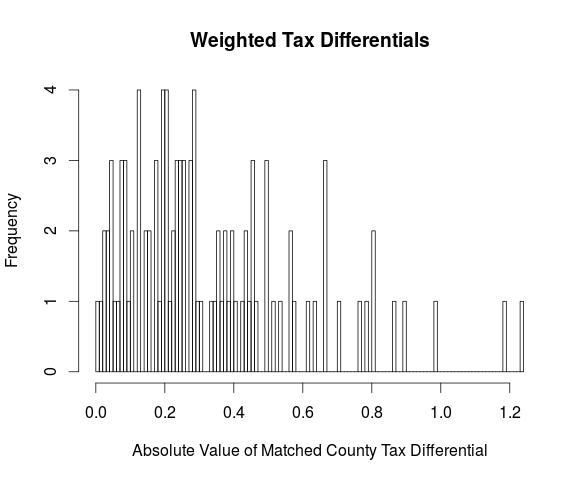
\includegraphics[scale=0.35]{taxdiff}
\end{figure}
\end{frame}

\begin{frame}
\frametitle{Some Comparisons Pt II}
Finally, we can rank average difference in firm start up rates and tax differential. Surprisingly we see that in the top 10 difference in mean start up rates along a state border, most of them share the same sign as the tax differential. Overall throughout our RD designs though, we find relatively low $R^{2}$ values.


\begin{table}[h]
\centering
\caption{Mean Firm Start Ups v Weighted Tax Differential}
{\tiny\renewcommand{\arraystretch}{.8}
\resizebox{\textwidth}{!}{%
\label{my-label}
\begin{tabular}{llll}
\hline \\[-1.8ex] 
Mean Firm Starts up & State Pair                      & Start up Favors & Tax Differential Favors \\
\hline \\[-1.8ex] 
1.642965            & Oklahoma - Texas                & Texas           & Oklahoma \\
1.621283            & New Mexico - Texas              & New Mexico      & New Mexico \\
1.548548            & Illinois - Missouri             & Missouri        & Missouri \\
1.546172            & Alabama - Georgia               & Alabama         & Alabama \\
1.435885            & California - Nevada             & Nevada          & Nevada \\
1.307654            & Indiana - Kentucky              & Kentucky        & Kentucky \\ 
1.257129            & North Carolina - South Carolina & South Carolina  & South Carolina \\
1.251866            & Oregon - Washington             & Oregon          & Oregon \\
1.233235            & North Carolina - Virginia       & Virginia        & Virginia \\
1.208313            & North Carolina - West Virginia  & North Carolina  & West Virginia \\
\hline
\end{tabular}}}
\end{table}

\end{frame}

\begin{frame}
\section{Conclusion}
\frametitle{Conclusion}
Going back to our original two research questions, we see that:
\begin{itemize}
\item Property, sales, and income taxes across most specifications besides for our interaction term regressions. 
\item Property tax rates have a relatively high elasticity, where a 1\% increase in relative property tax rates corresponds to a 0.49\% decrease in relative firm start up rates.
\item This may be due to many firms being small, and so individuals on one side of the border (with preferential government expenditures) can start up a business in the neighboring county. No good explanation for stability across naics subfields.
\item Government expenditures on infrastructure, welfare, and education does not seem to impact firm start up rates

\end{itemize}
\end{frame}

\begin{frame}
\frametitle{Future Work or Extensions}
\begin{itemize}
\item Can we find ways to proxy or estimate location specific heterogeneity? Calculating agglomeration figures for every county as a first attempt, county level tax rates (very hard to get). Etc.
\item Testing coefficients as we get further away from the border (match counties on opposite ends of the state, test for state fixed effects, etc). Currently in the works!
\item Run estimator over sub samples of counties of different sizes as a way to better control for "distance."
\end{itemize}
\end{frame}

\begin{frame}
\begin{centering}
\huge{Thank you for your time!}
\end{centering}
\end{frame}
\end{document}